
%
%  void-input - easy report template for included file
%  EDIT THE LINE ABOVE FOR DOCUMENTATION OF THIS FILE, then delete this line! 
%         

%

% ============================================================
% --- texstudio magic comment: 
% !TEX encoding = UTF-8
% !TeX program = pdflatex
%% !TeX program = xelatex
% !TeX root = "cognome-tesina.tex"
% %  !TeX spellcheck = en_US
% !TeX spellcheck = it_IT


% ====================================================================


\chapter{Task 1}
This task was very simple. Even with my little prior knowledge of c++ I had no difficulty doing it. In fact, it was enough to add some if statements and some basic OpenCV functions to complete it.

\chapter{Task 2}
Like the previous task, there were no problems with this one either. I simply used .channels() to find the channels of the image and then print them to the screen. While for cv::waitKey() I used a variable.



\chapter{Task 3}
I performed the third task differently from what was suggested on the slides using the cv::Mat::zeros function (found on internet) to set the channel values to 0. I then divided the image channels and used the function to bring to zero the indicated channels and then I did a merge of the channels to reconstruct the image.

\begin{figure}[h]
	\centering
	\begin{minipage}{0.45\textwidth}
		\centering
		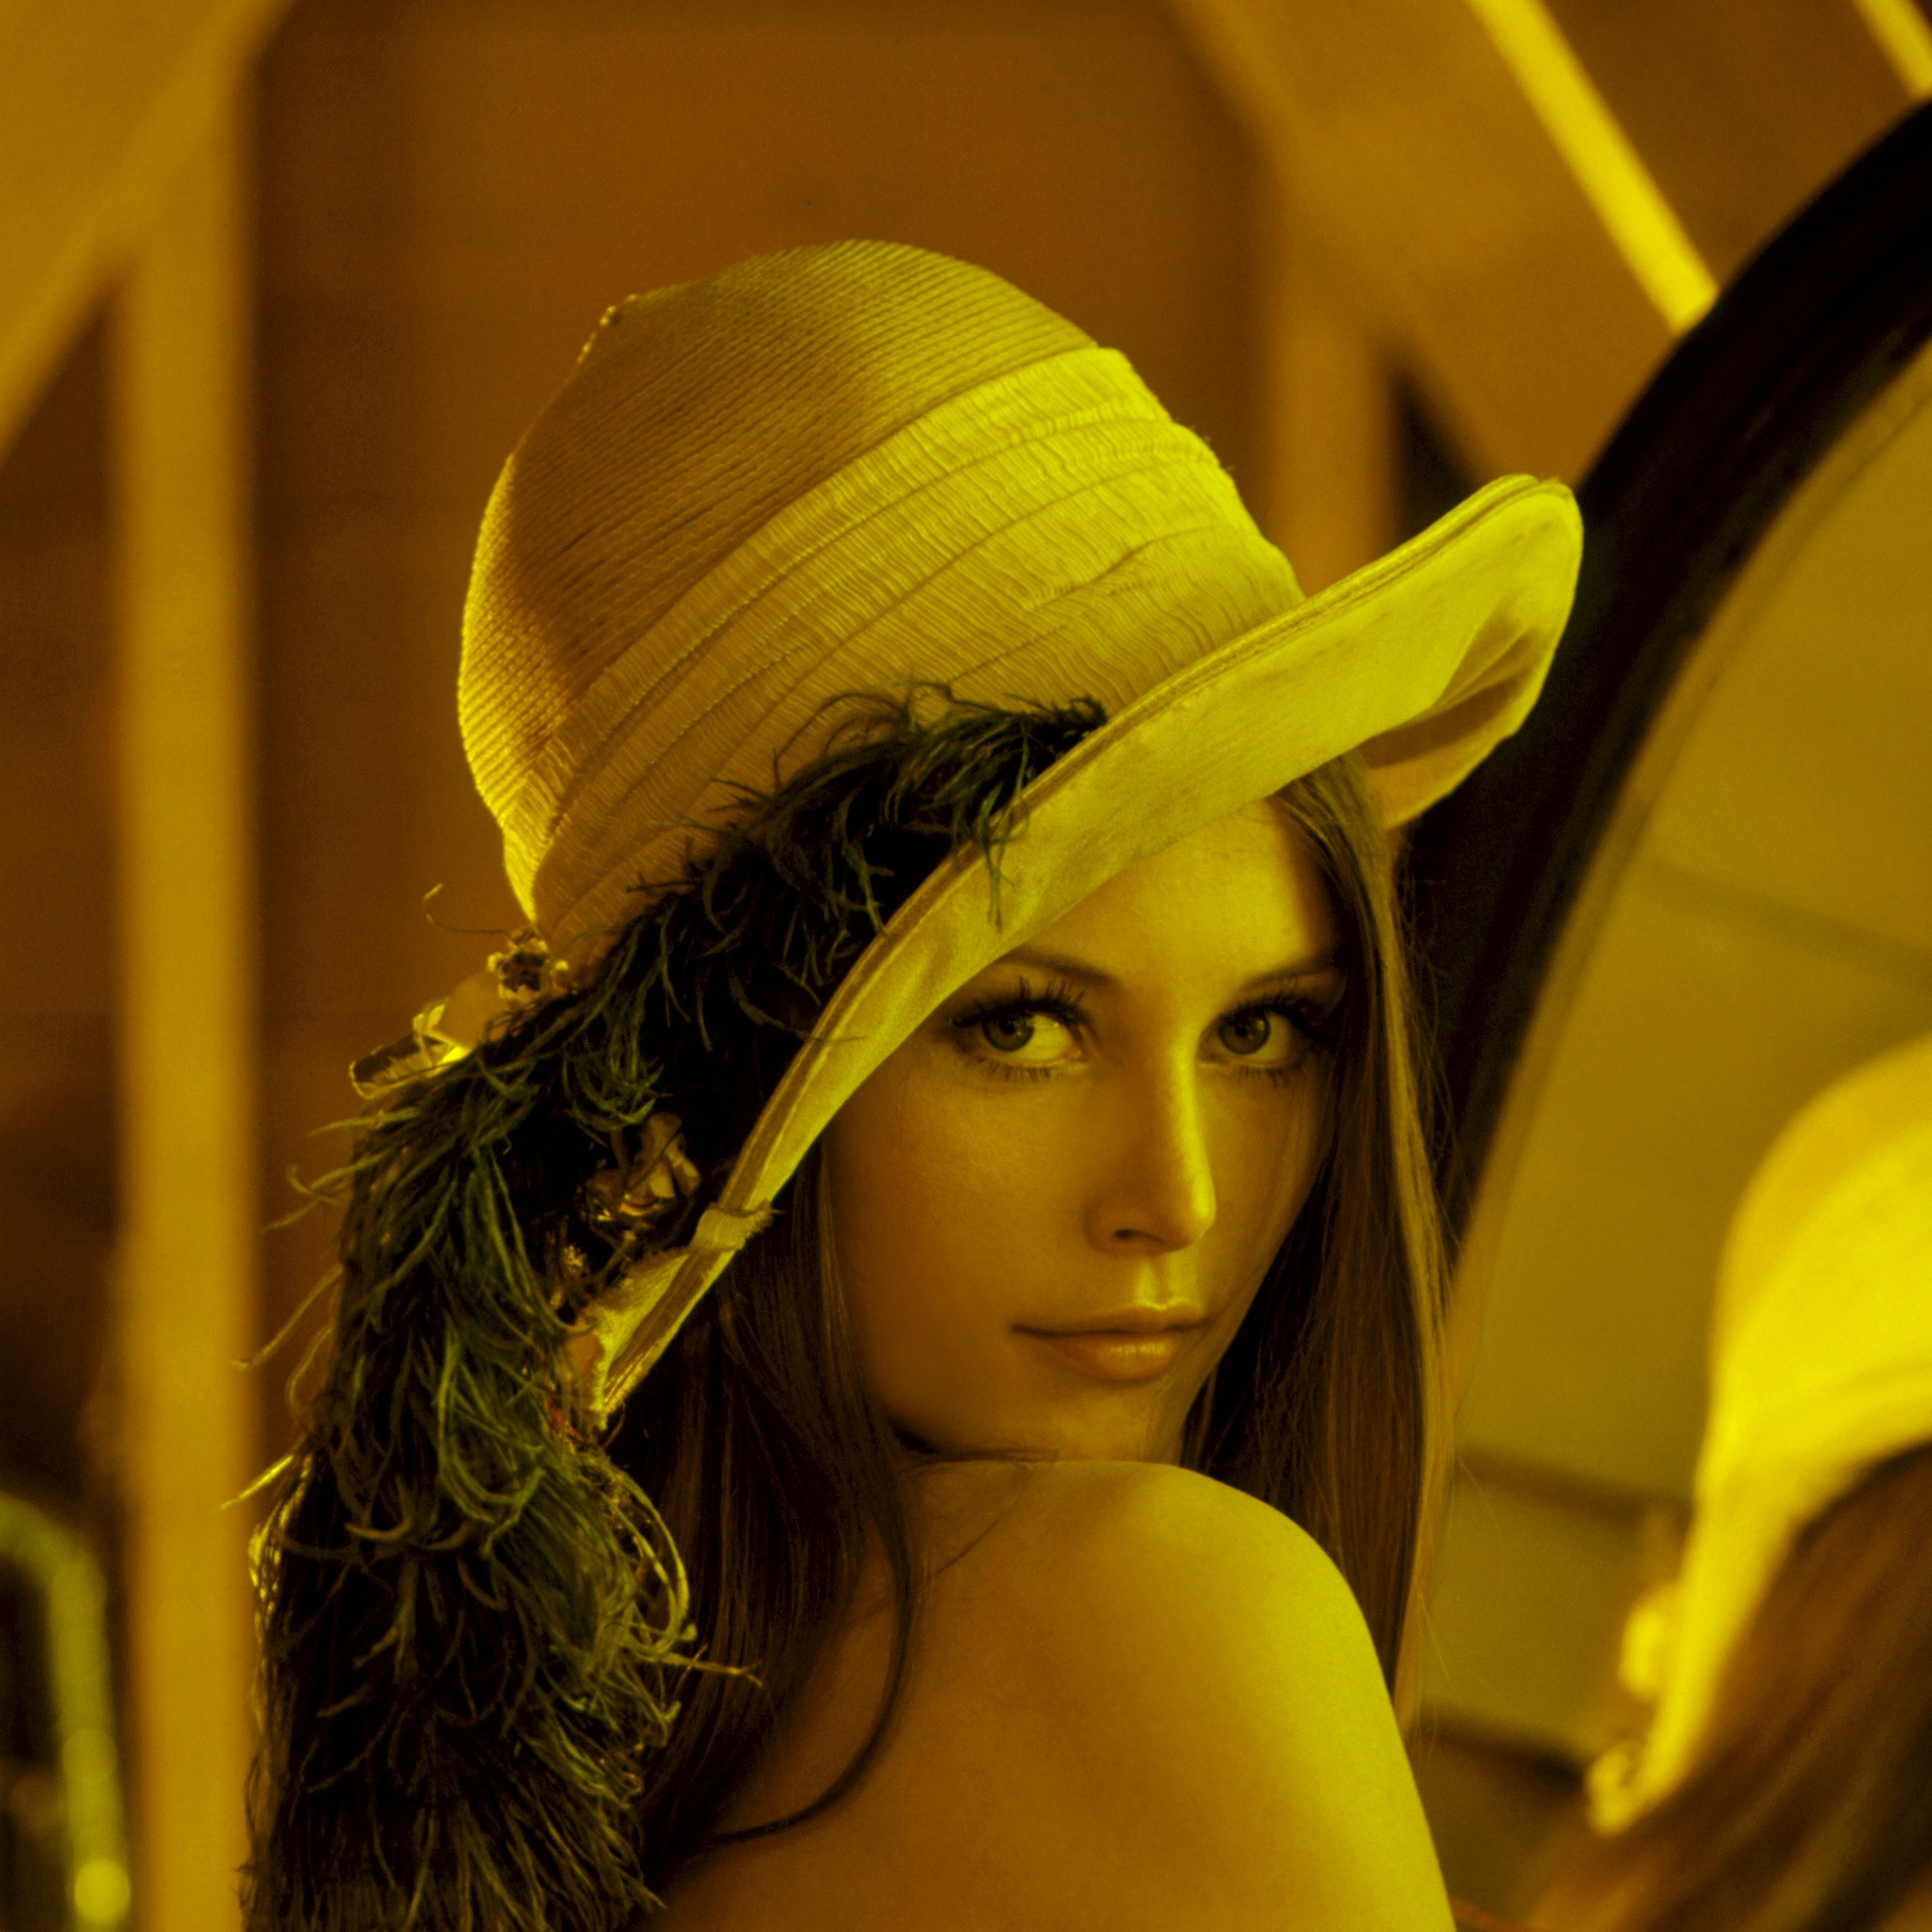
\includegraphics[width=\linewidth]{images/source/task3/1}
		\caption{Lena\_color without channel 0}
		\label{fig:1a}
        \end{minipage}
        \hspace{0.05\textwidth}
        \begin{minipage}{0.45\textwidth}
        		\centering
		
\includegraphics[width=\linewidth]{images/source/task3/2}
		\caption{Lena\_grayscale without channel 1}
		\label{fig:1b}
        \end{minipage}
\end{figure}

\begin{figure}[!h]
	\centering
	\begin{minipage}{1\textwidth}
		\centering
		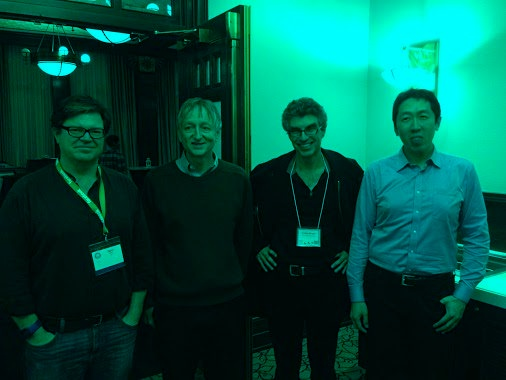
\includegraphics[scale=0.25]{images/source/task3/3}
		\caption{DL\_gurus without channel 2}
		\label{fig:1}
	\end{minipage}
\end{figure}


\chapter{Task 4}
With the fourth exercise I used the same technique and consequently I didn't encounter any major difficulties.

\begin{figure}[h]
	\centering
	\begin{minipage}{0.45\textwidth}
		\centering
		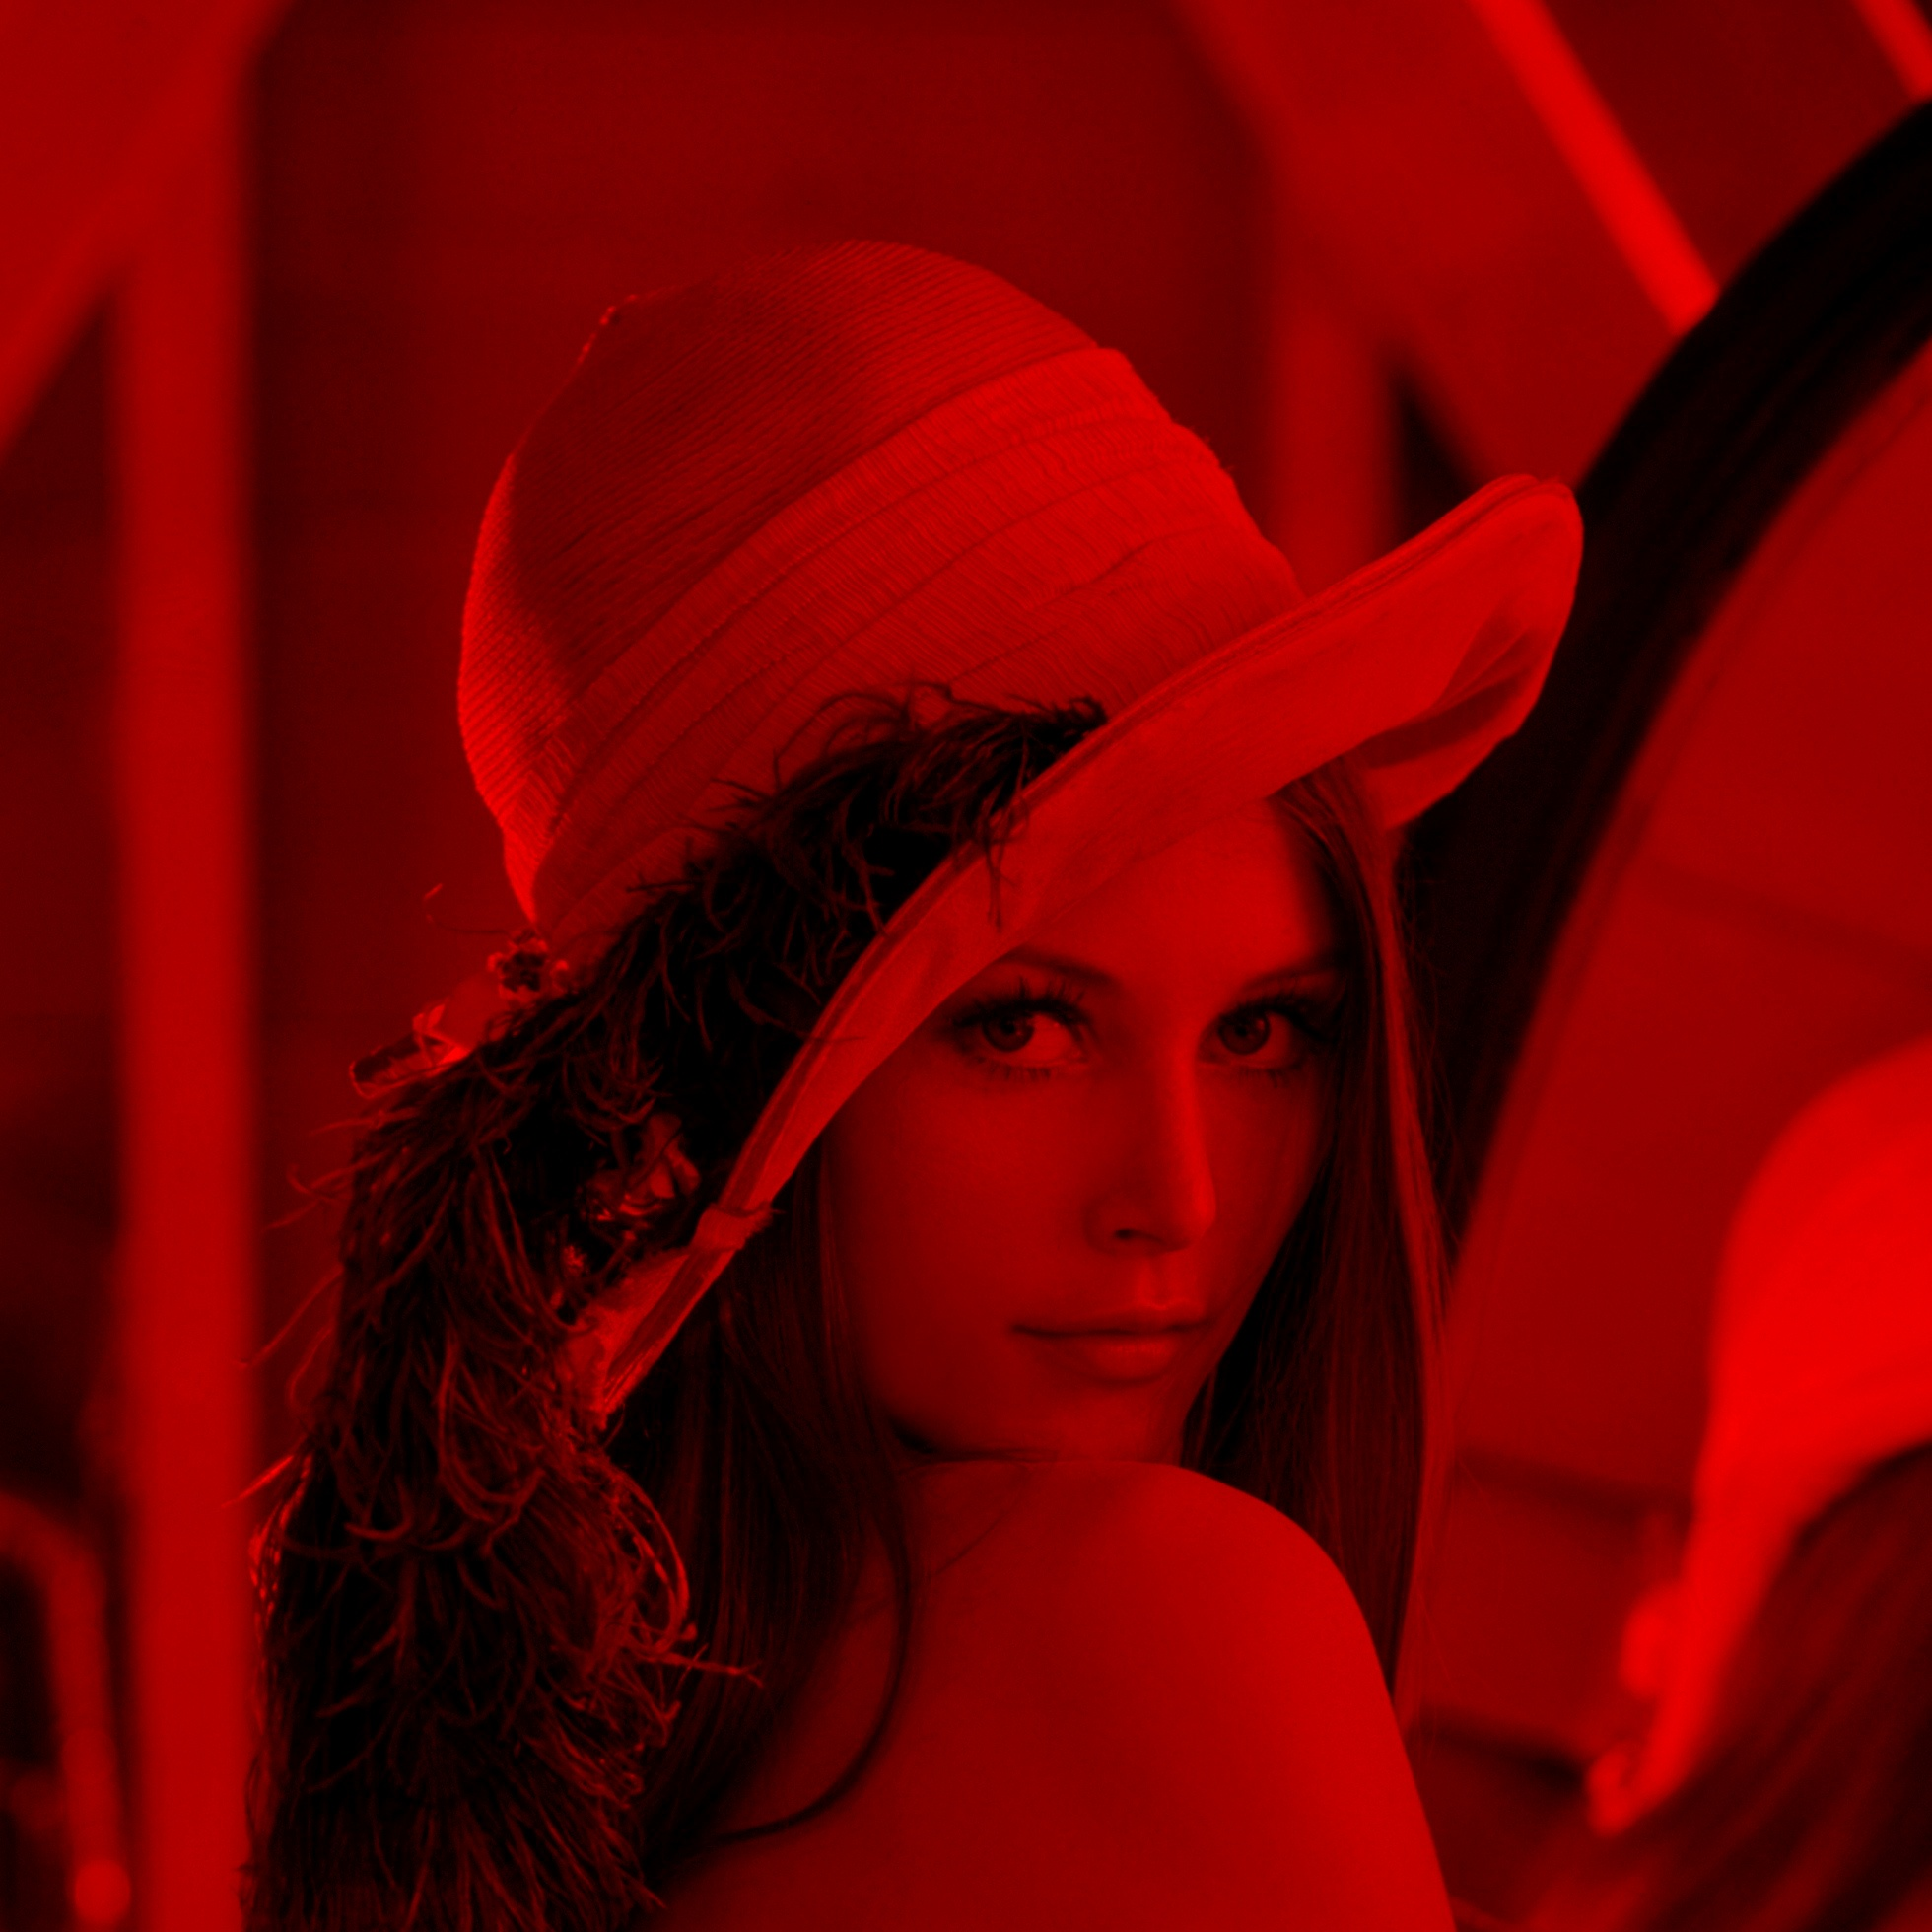
\includegraphics[width=\linewidth]{images/source/task4/1/1}
		\caption{Lena\_color red channel}
		\label{fig:1a}
        \end{minipage}
        \hspace{0.05\textwidth}
        \begin{minipage}{0.45\textwidth}
        		\centering
		
\includegraphics[width=\linewidth]{images/source/task4/1/2}
		\caption{Lena\_color green channel}
		\label{fig:1b}
        \end{minipage}
        \hspace{0.05\textwidth}
        \begin{minipage}{0.45\textwidth}
        		\centering
		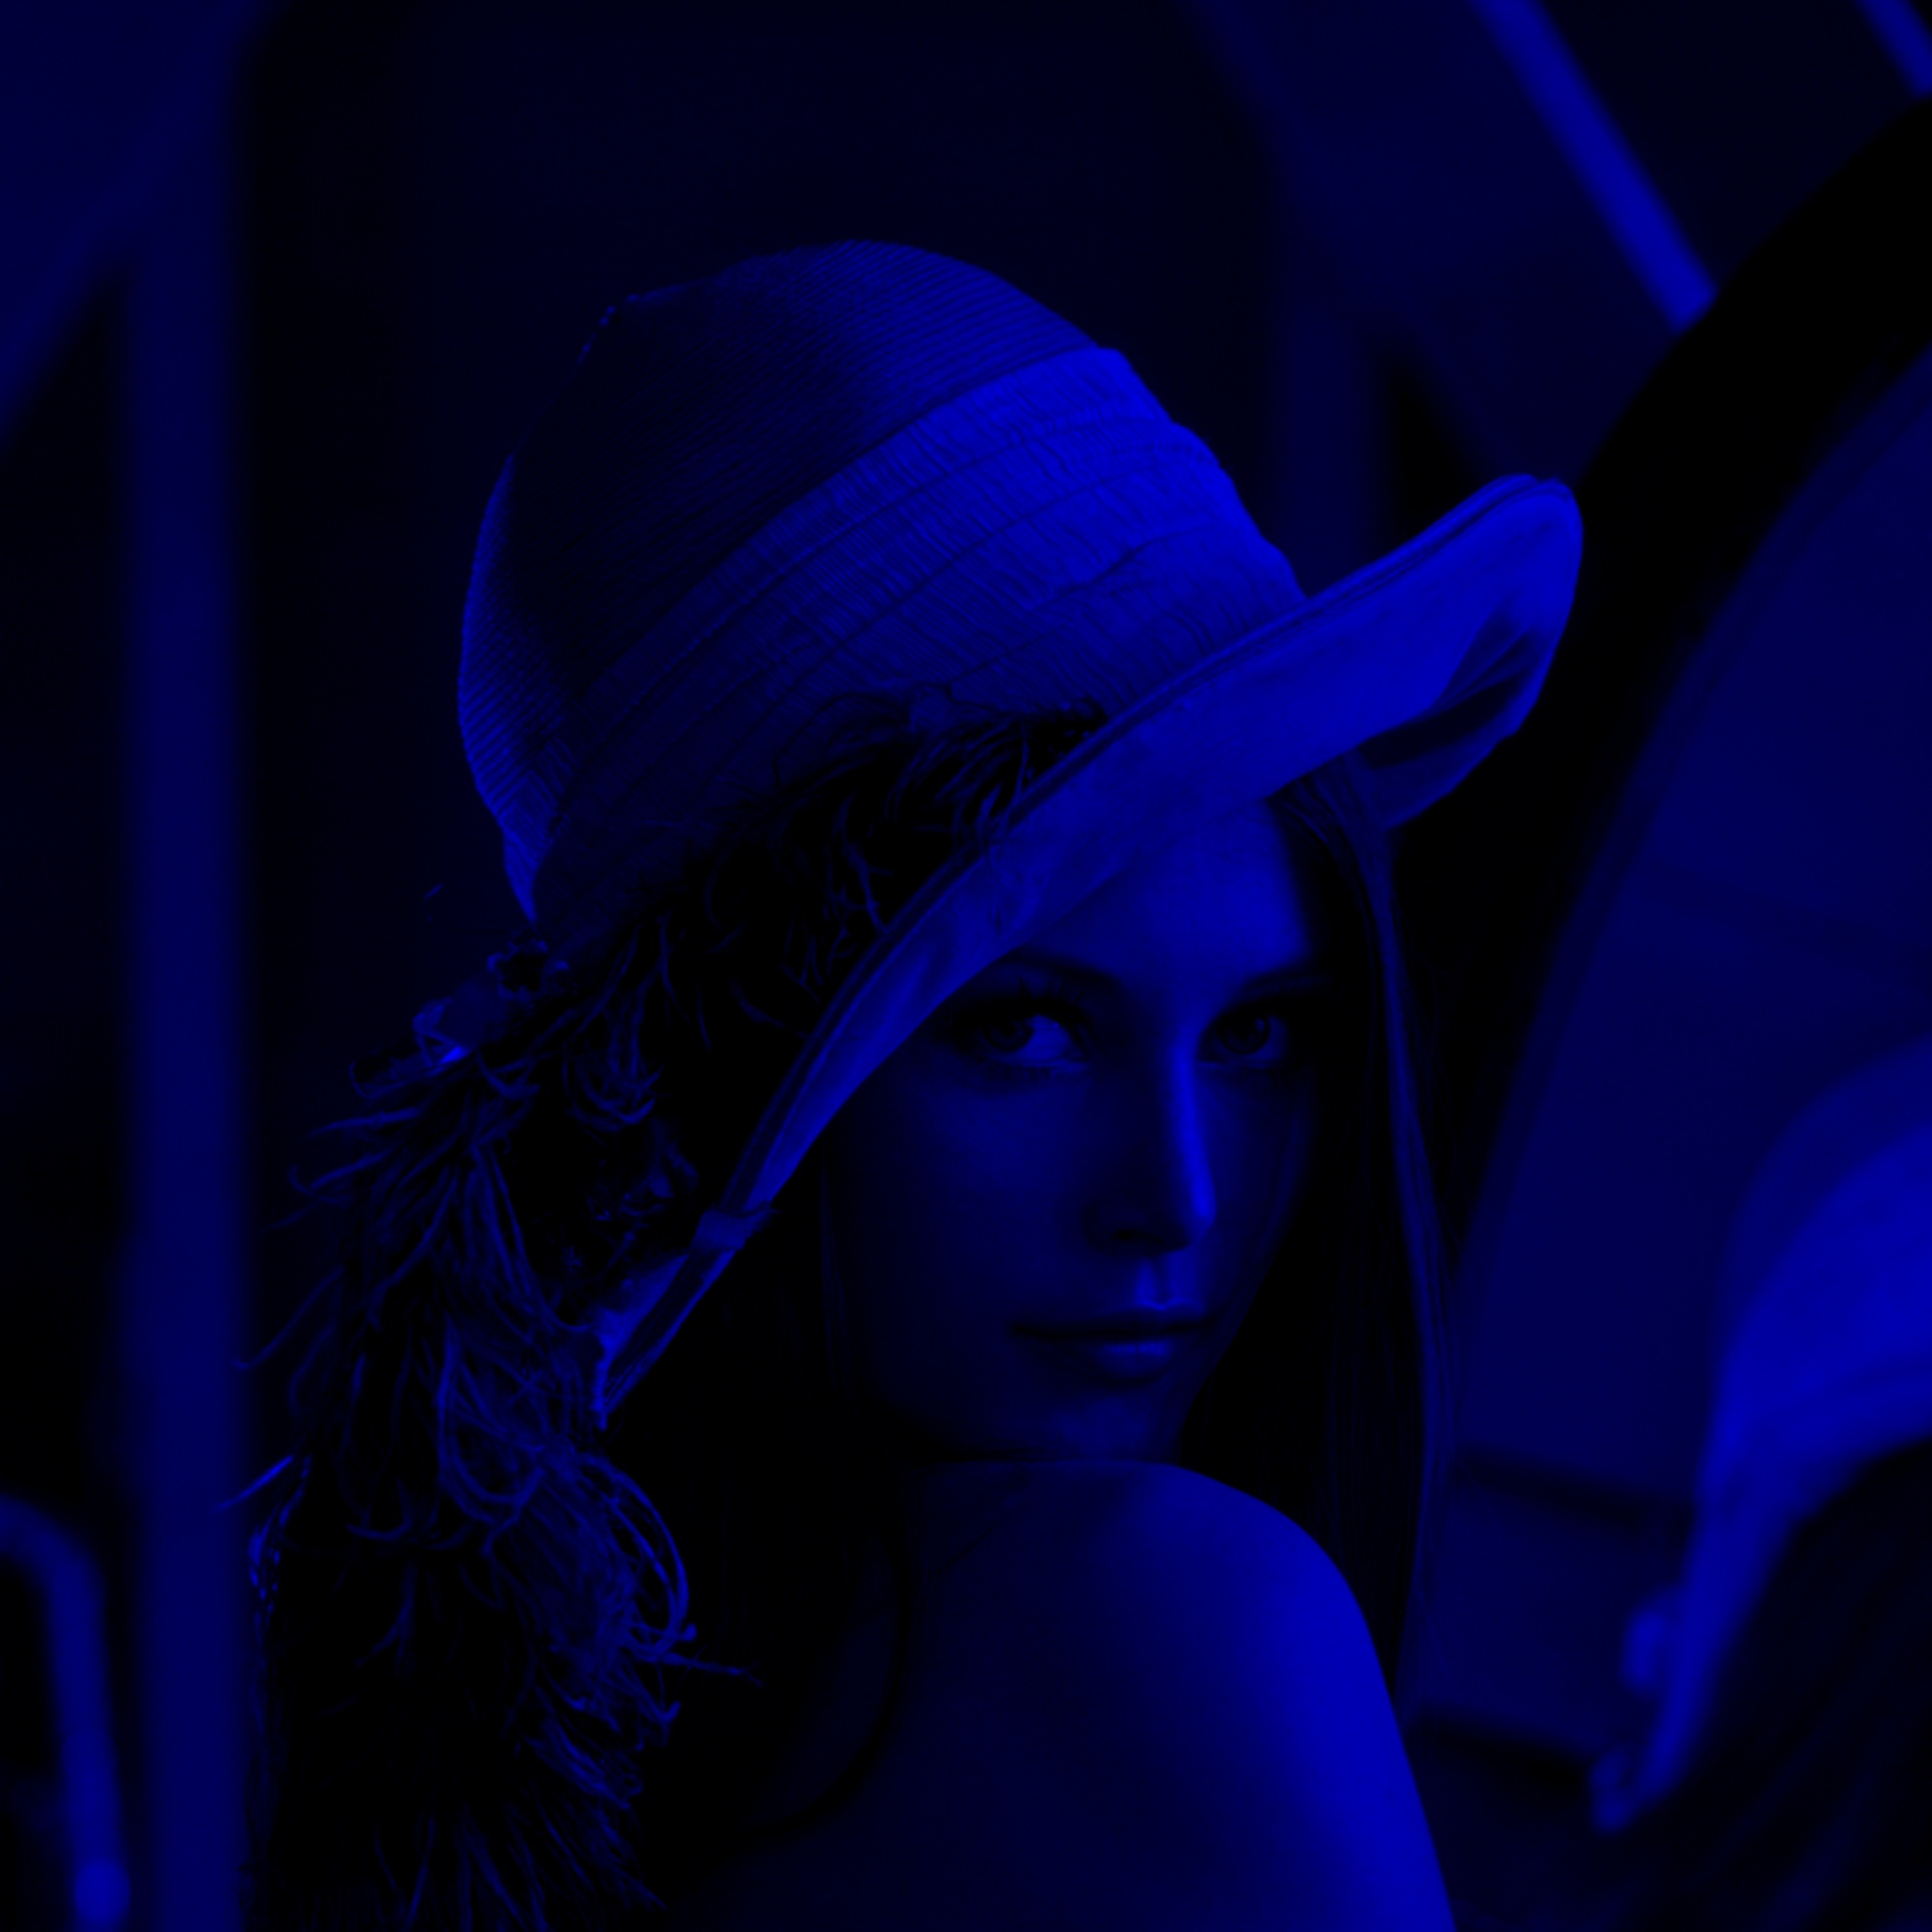
\includegraphics[width=\linewidth]{images/source/task4/1/3}
		\caption{Lena\_color blue channel}
		\label{fig:1b}
        \end{minipage}
\end{figure}

\begin{figure}[h]
	\centering
	\begin{minipage}{0.45\textwidth}
		\centering
		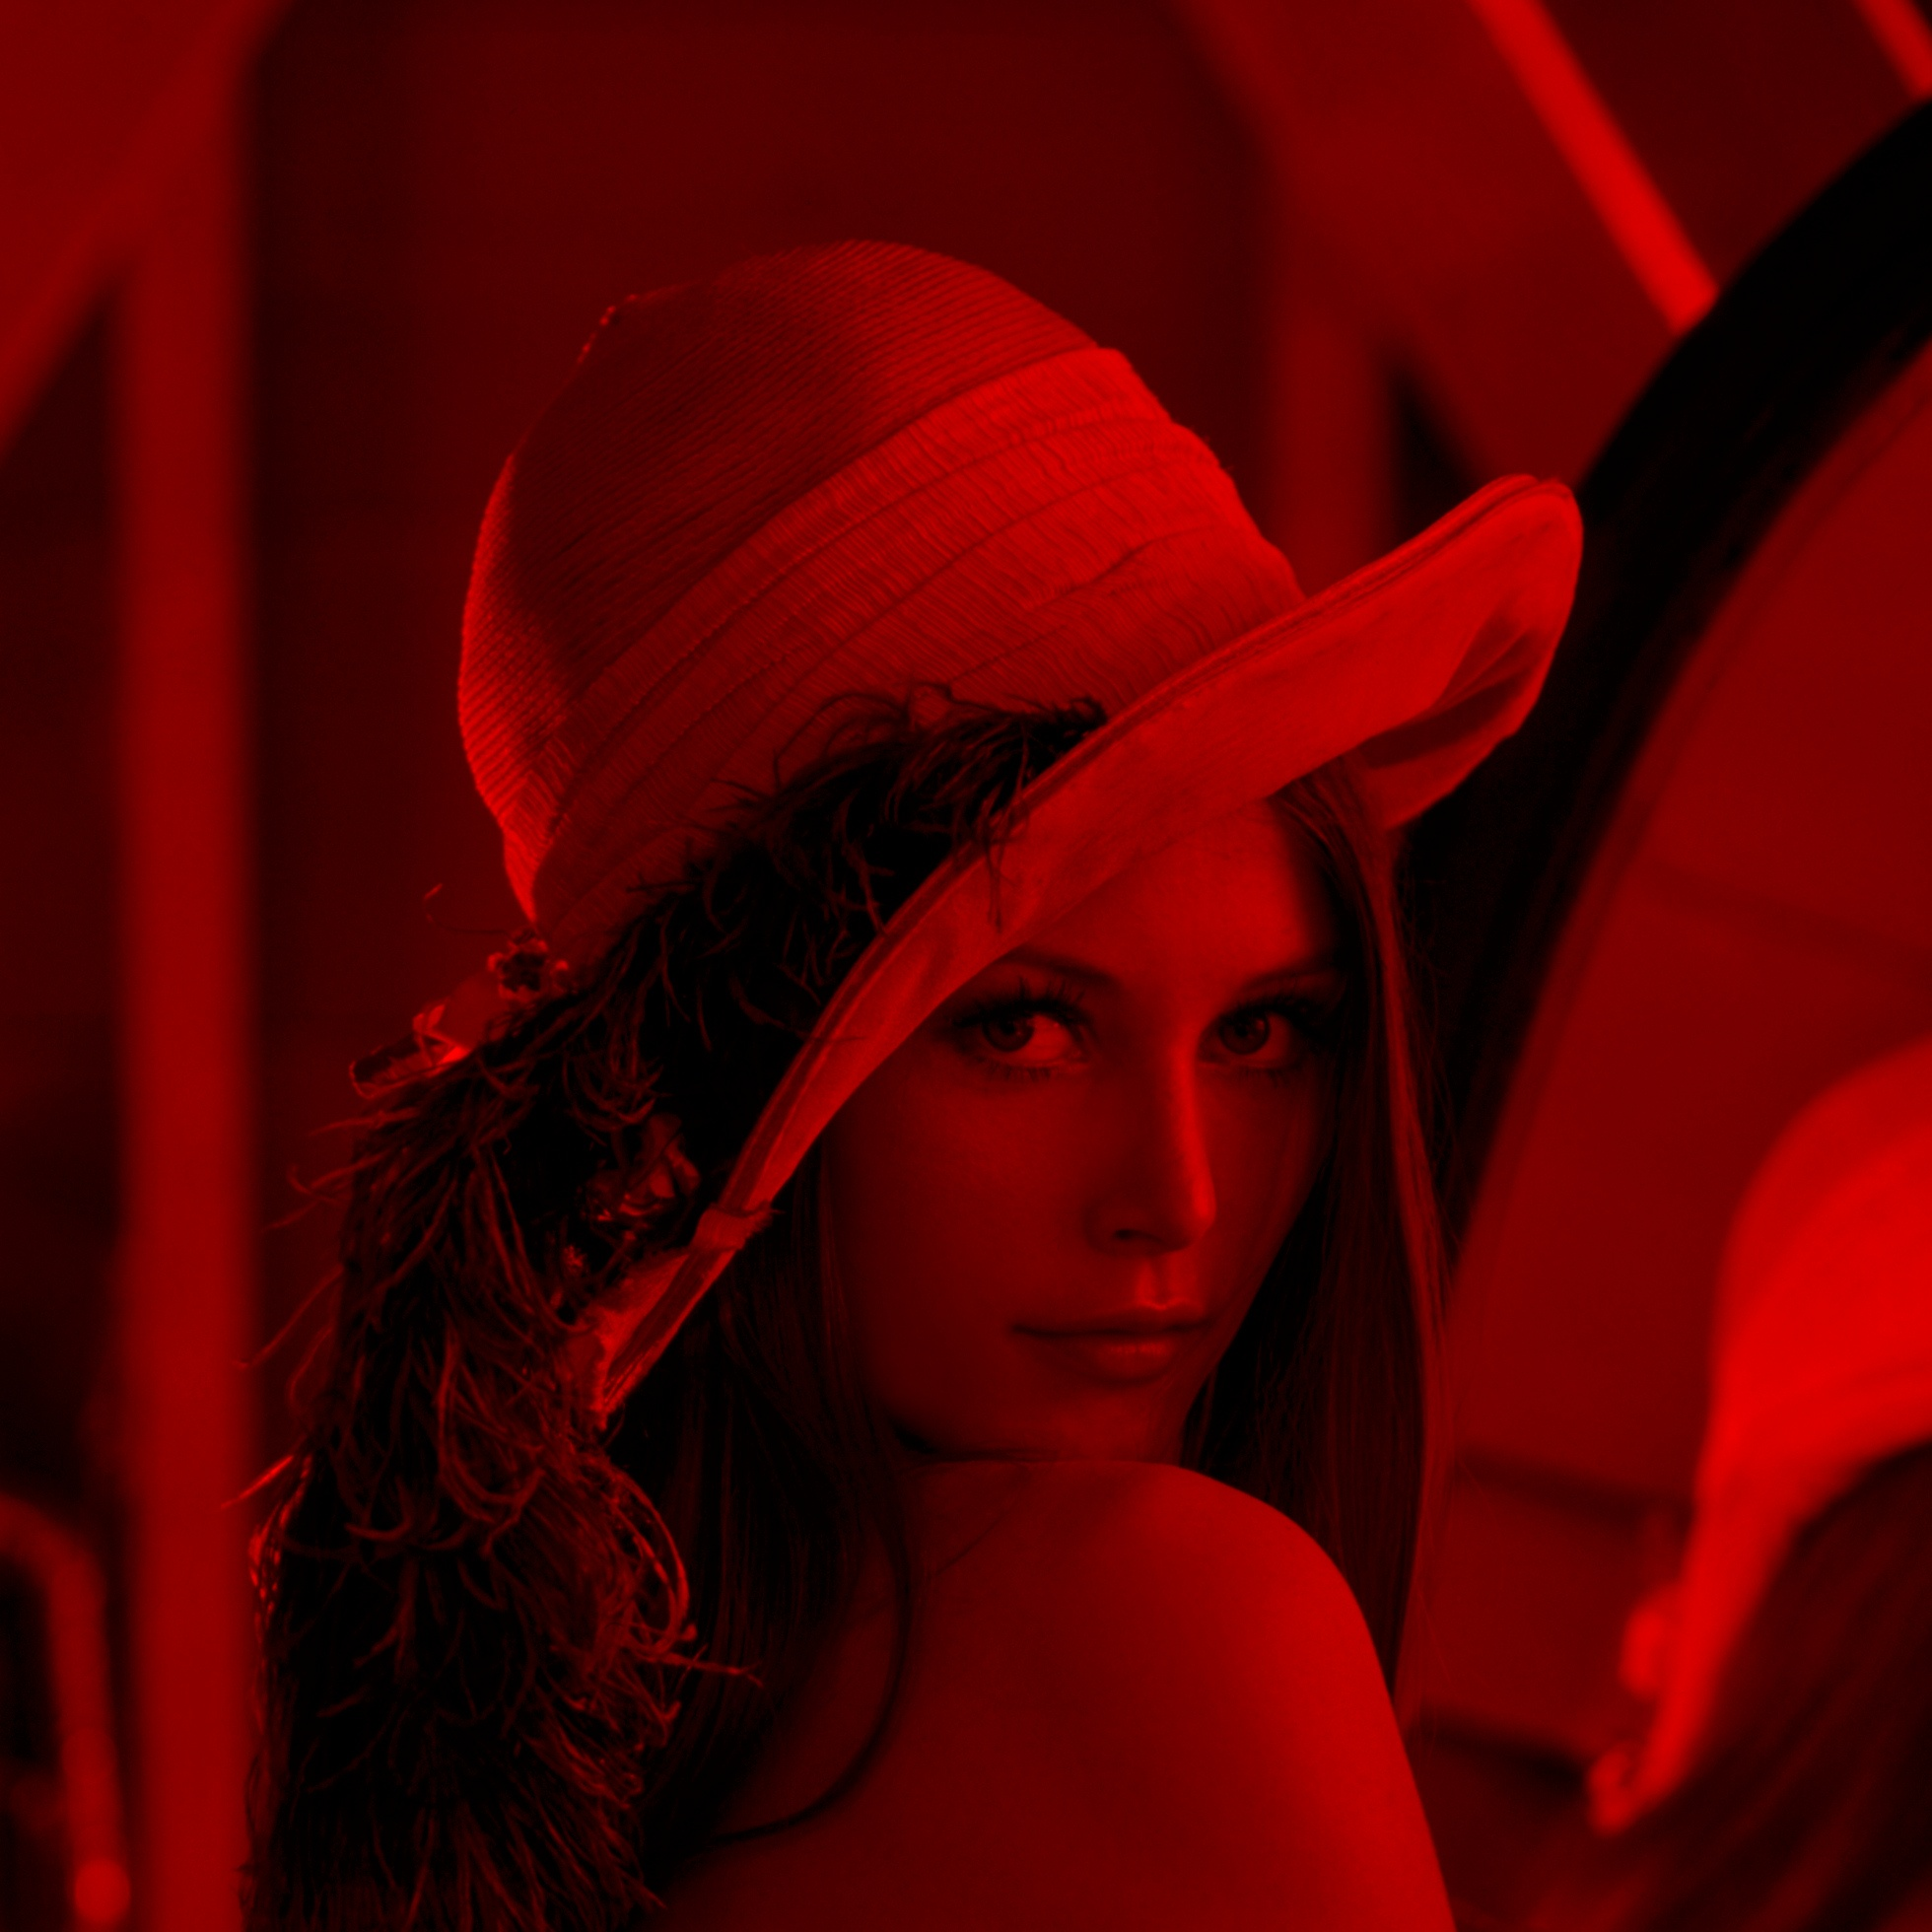
\includegraphics[width=\linewidth]{images/source/task4/2/1}
		\caption{Lena\_grayscale red channel}
		\label{fig:1a}
        \end{minipage}
        \hspace{0.05\textwidth}
        \begin{minipage}{0.45\textwidth}
        		\centering
		
\includegraphics[width=\linewidth]{images/source/task4/2/2}
		\caption{Lena\_grayscale green channel}
		\label{fig:1b}
        \end{minipage}
        \hspace{0.05\textwidth}
        \begin{minipage}{0.45\textwidth}
        		\centering
		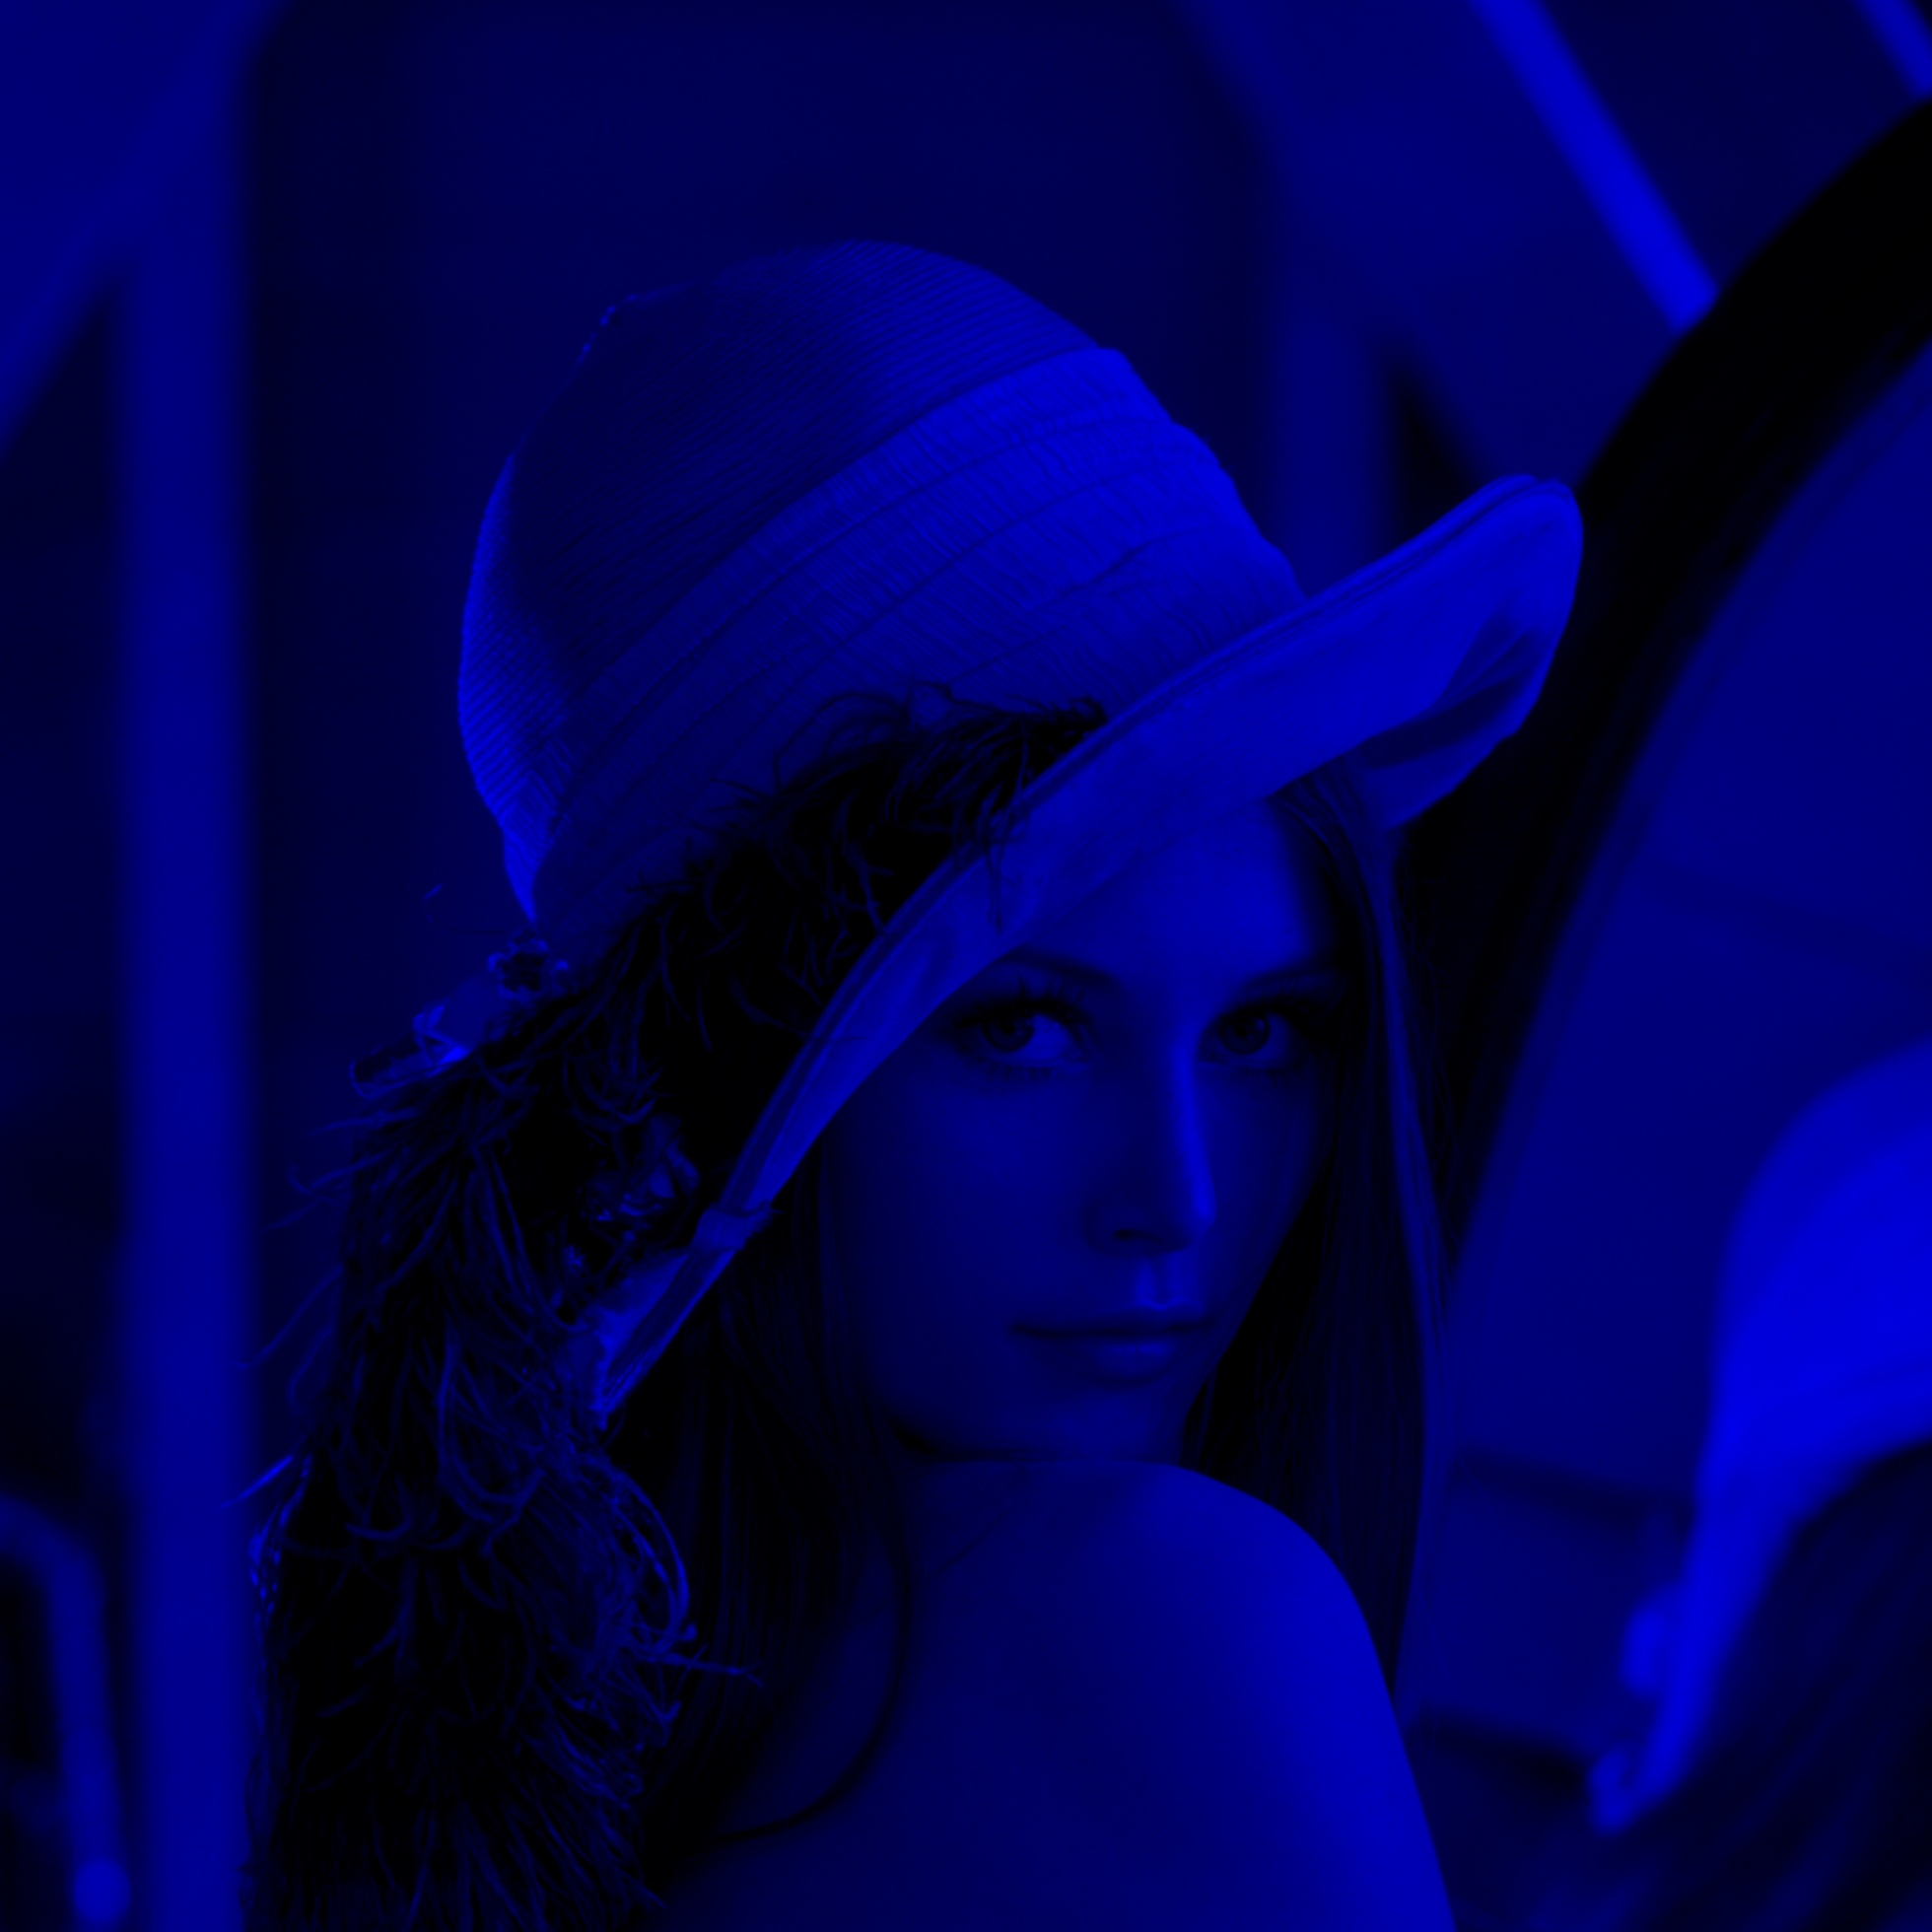
\includegraphics[width=\linewidth]{images/source/task4/2/3}
		\caption{Lena\_grayscale blue channel}
		\label{fig:1b}
        \end{minipage}
\end{figure}

\begin{figure}[h]
	\centering
	\begin{minipage}{0.45\textwidth}
		\centering
		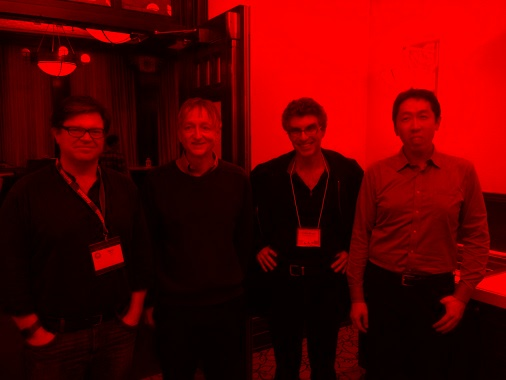
\includegraphics[width=\linewidth]{images/source/task4/3/1}
		\caption{DL\_gurus red channel}
		\label{fig:1a}
        \end{minipage}
        \hspace{0.05\textwidth}
        \begin{minipage}{0.45\textwidth}
        		\centering
		
\includegraphics[width=\linewidth]{images/source/task4/3/2}
		\caption{DL\_gurus green channel}
		\label{fig:1b}
        \end{minipage}
        \hspace{0.05\textwidth}
        \begin{minipage}{0.45\textwidth}
        		\centering
		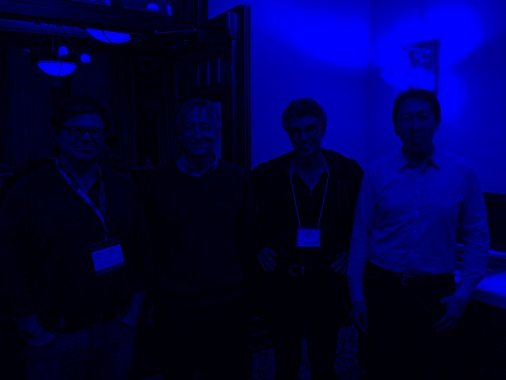
\includegraphics[width=\linewidth]{images/source/task4/3/3}
		\caption{DL\_gurus blue channel}
		\label{fig:1b}
        \end{minipage}
\end{figure}


\chapter{Task 5}
With the fifth exercise after some initial failed tests I understood that it is simply enough to use the for loops to tell it how to color the pixels. So the problem was more of logic than of carrying out the exercise.
Once I understood this, the implementation of the code was very fast.

\begin{figure}[h]
	\centering
	\begin{minipage}{0.45\textwidth}
		\centering
		
\includegraphics[width=\linewidth]{images/source/task5/1}
		\caption{Vertical gradient}
		\label{fig:1a}
        \end{minipage}
        \hspace{0.05\textwidth}
        \begin{minipage}{0.45\textwidth}
        		\centering
		
\includegraphics[width=\linewidth]{images/source/task5/2}
		\caption{Horizontal gradient}
		\label{fig:1b}
        \end{minipage}
\end{figure}

\begin{figure}[h]
	\centering
	\begin{minipage}{0.45\textwidth}
		\centering
		
\includegraphics[width=\linewidth]{images/source/task5/3}
		\caption{chessboard with squares of size 20 pixels}
		\label{fig:1a}
        \end{minipage}
        \hspace{0.05\textwidth}
        \begin{minipage}{0.45\textwidth}
        		\centering
		
\includegraphics[width=\linewidth]{images/source/task5/4}
		\caption{chessboard with squares of size 50 pixels}
		\label{fig:1b}
        \end{minipage}
\end{figure}



% ====================================================================

% ====================================================================
% memo available commands
% ====================================================================
% easyrep: summary of provided macros
%
% \Title{text}     defines the document title 
% \Subtitle{text}  defines the subtitle
% \Author{text}    defines the author string
% \Date{text}      defines a date string
% \printCover      print a cover page using above information
%
% --- text styles
% \tDef{text}      definition (generic) 
% \tDefObj{text}   definition (the ter being defined)
% \tDefTxt{text}   definition (the statement defining the term) 
% \tRemark{text}   remarked text
% \tREMARK{text}   highly remarked text 
% \tLoud{text}     shouted text! 
% \tCode{text}     inline code text
% \tLatin{text}    latin text
% \tForeign{text}  foreign language text 
% \tExample{text}  example 
% \tStandard{text} a recommendation 
% \tQuote{text}    a quoted text 
% \tQuoteFig{text} a quoted text referring to a figure 
% \tConcept{text}  an important concept  
% \tBeginPar{text} highlighted text 
%                  at the beginning of a paragraph 
%
% ---environments
% \begin{quoteStandard} text... \end{quoteStandard}
%    print text to be quoted, e.g. sentences from 
%    a recommendation
%
% \begin{quoteRemark} text... \end{quoteRemark}
%    similar to quoteStandrd, but the text is more marked
%
%  
% --- typo accelerators
% \qmo             opening quotation mark (use \qmo{})
% \qmc             closing quotation mark (use \qmc{})
% \th  emphasises "th"
% \ie  slanted "i.e."
% \eg  slanted "e.g."
% \es  slanteg "ad es."
% \octave   "octave" in \tCode style
% \matlab   "matlab"
% \labview  "labVIEW"
% \latex    "LaTeX" (just the text!)
%
% --- math typo accelerators
% \v{math text}  underlines the math text (useful for vector) 
%
% --- debug commands
% \debugTextStyles        print a table showing text styles
% \debugPrintCharacters   print a table of characters
% \Vispa                  print some text (to fill)  
% \Vispas                 more filling text
% ====================================================================
